\renewcommand{\chaptername}{March 8th: Lab}
\chapter{Qubits and Quantum Circuits}

%Python library with tools to facilitate simulation of quantum systems
Conventionally, information is stored in bits, as a series of 0s and 1s. However, in quantum computing `quantum bits', or simply `qubits', are used. These obey the rules of quantum mechanics and allow for information to be processed in new and different ways. %qubits are the fundamental unit of computation in a quantum computer
%A qubit (or quantum bit) is the quantum mechanical analogue of a classical bit. In classical computing the information is encoded in bits, where each bit can have the value zero or one. In quantum computing the information is encoded in qubits. A qubit is a two-level quantum system

In order to manipulate these qubits (i.e. change them between quantum states) `quantum gates' can be applied to build a `quantum circuit'. A quantum circuit is a computational routine consisting of coherent quantum operations on quantum data, such as qubits, and concurrent real-time classical computation. It is an ordered sequence of quantum gates, measurements and resets, all of which may be conditioned on and use data from the real-time classical computation.

\section{Objectives}
The purpose of this lab is to investigate quantum bits and quantum circuits using `qiskit`. Thus, the following objectives were pursued:
\begin{itemize}
    \item Become familiar with `qiskit'
    \item Implement quantum gates and visualise the state of a qubit through the Bloch sphere
    \item Obtain deeper understanding of quantum operations and quantum circuits basics
\end{itemize}

\section{Methods}
Quantum circuits were implemented and visualised using python in Jupyter Notebook -- a web-based interactive computational environment for programming languages. Specifically, a library named `qiskit' was used -- an open-source software development kit for working with quantum computers. It provides tools for creating quantum programs and for running them on simulators on a local computer. 

The Aer simulator was used to simulate realistic quantum systems with realistic noise models.

To evaluate the rigidity of the analytical predictions from qiskit, the circuits were built on protoype quantum devices provided by IBM Quantum. `The IBM Quantum Composer' is an online platform allowing public access to remote quantum computing services.

\section{Results}
Qubits can be represented by 2D vectors, their states are limited to the form:

$$ |q\rangle = \cos{\tfrac{\theta}{2}}|0\rangle + e^{i\phi}\sin{\tfrac{\theta}{2}}|1\rangle $$
where $\theta$ and $\phi$ are real numbers. 

This state can be visualized using a `Bloch Sphere' (a geometrical representation of a two-level qubit) and quantum gates can be used to manipulate the state. These gates can be represented as matrices, and as rotations around the Bloch sphere.

In this lab report, Pauli gates, the Hadamard gate and some Multi-qubit gates are analysed.
%A normal logic gate gets a simple set of inputs and produces one definite output. A quantum gate manipulates an input of superpositions, rotates probabilities, and produces another superposition as its output.

\subsection{The Pauli Gates}

\subsubsection{The X Gate}
The X gate is represented by the Pauli-X matrix:

$$ X = \begin{bmatrix} 0 & 1 \\ 1 & 0 \end{bmatrix} = |0\rangle\langle1| + |1\rangle\langle0| $$

A circuit was created to determine the effect an X gate has on a qubit. A qubit was initialised in state $|0\rangle$ and passed through an X gate, the circuit diagram of which is shown in Figure \ref{fig:xGate}.

\begin{figure}[h]
    \centering
    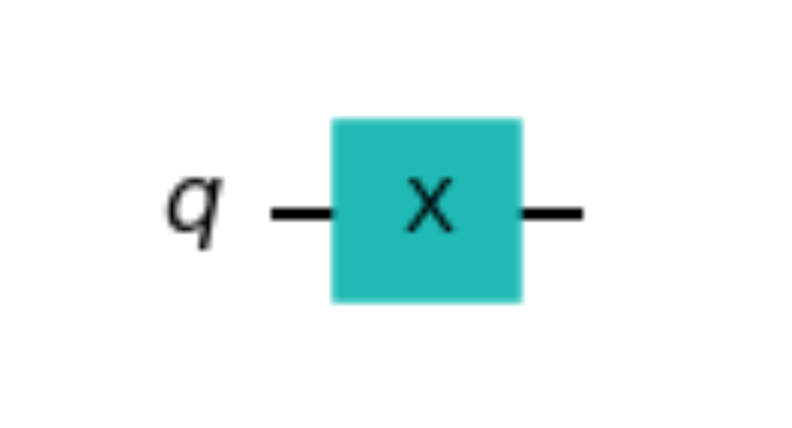
\includegraphics[width=0.3\textwidth]{lab2/images/xGate.png}
    \caption{Circuit diagram of a Pauli-X gate} 
    \label{fig:xGate}
\end{figure}

From the mathematics, it is clear that applying an X gate switches the amplitudes of the states $|0\rangle$ and $|1\rangle$:

$$ X|0\rangle = \begin{bmatrix} 0 & 1 \\ 1 & 0 \end{bmatrix}\begin{bmatrix} 1 \\ 0 \end{bmatrix} = \begin{bmatrix} 0 \\ 1 \end{bmatrix} = |1\rangle \quad\quad\quad\quad
X|1\rangle = \begin{bmatrix} 0 & 1 \\ 1 & 0 \end{bmatrix}\begin{bmatrix} 0 \\ 1 \end{bmatrix} = \begin{bmatrix} 1 \\ 0 \end{bmatrix} = |0\rangle$$

%DEMONSTRATED
The circuit (shown in Figure \ref{fig:xGate}) was constructed using qiskit and the states were observed using a Bloch sphere which is seen in Figure \ref{fig:bSphereXGate}. The X gate performed a rotation by $\pi$ around x-axis of the Bloch sphere (the qubit switched to state $|1\rangle$ after being initialised in state~$|0\rangle$).

\begin{figure}[h]
    \centering
    \begin{subfigure}[h]{0.33\textwidth}
        \centering
        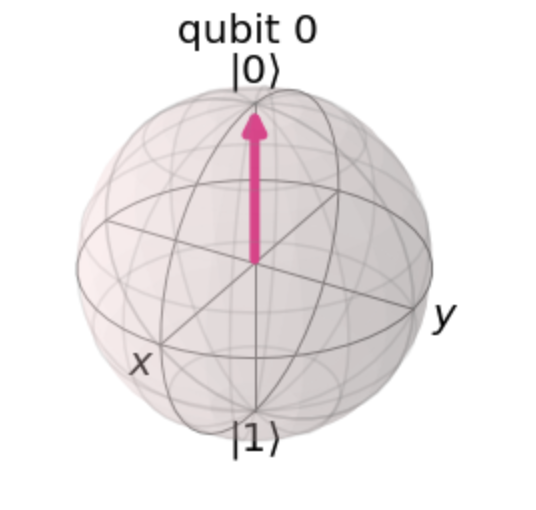
\includegraphics[width=\textwidth]{lab2/images/bSphX1.png}
        \caption{}
        \label{fig:bSphX1}
    \end{subfigure}
    \hspace{0.2\textwidth}
    \begin{subfigure}[h]{0.33\textwidth}
        \centering
        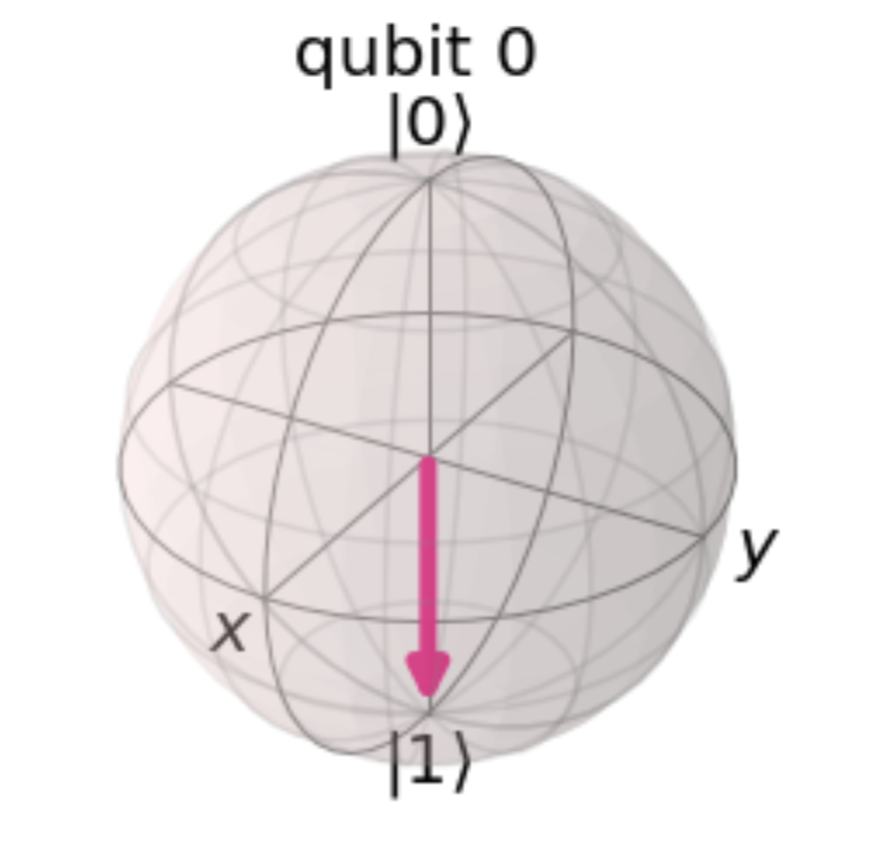
\includegraphics[width=\textwidth]{lab2/images/bSphX2.png}
        \caption{}
        \label{fig:bSphX2}
    \end{subfigure}
    \caption{Bloch sphere showing a) the state of the initialised qubit and b) the state of the qubit after being passed through a Pauli-X gate} 
    \label{fig:bSphereXGate}
\end{figure}

\subsubsection{The Y and Z gates}

Similar to the X gate, the Y and Z Pauli matrices can represent the Y and Z gates in our quantum circuits. These gates perform rotations by $\pi$ around the y and z-axis of the Bloch sphere, respectively.

$$ Y = \begin{bmatrix} 0 & -i \\ i & 0 \end{bmatrix} = -i|0\rangle\langle1| + i|1\rangle\langle0| $$

$$ Z = \begin{bmatrix} 1 & 0 \\ 0 & -1 \end{bmatrix} = |0\rangle\langle0| - |1\rangle\langle1| $$

A circuit was created with an X and Y gate in series, as shown in Figure \ref{fig:xyGateDiagram}.

\begin{figure}[h]
    \centering
    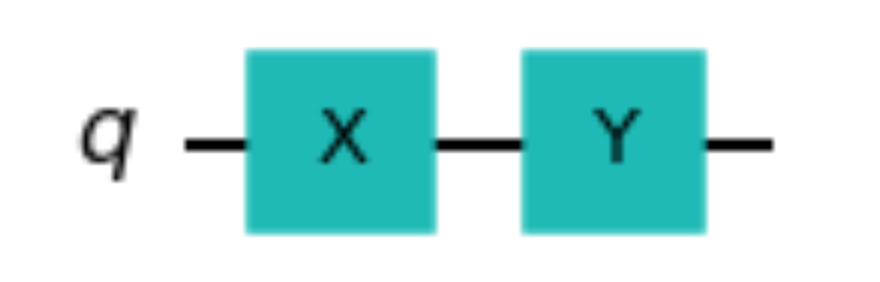
\includegraphics[width=0.3\textwidth]{lab2/images/xyGate.png}
    \caption{Circuit diagram of Pauli-X gate followed by a Pauli-Y gate in series} 
    \label{fig:xyGateDiagram}
\end{figure}

The resultant state was observed through the use of a Bloch sphere. After passing through circuit described in Figure \ref{fig:xyGateDiagram}, the qubit was found to be in state $|0\rangle$ -- seemingly unchanged from its initialised state -- as seen in Figure \ref{fig:xyGateBloc}.

\begin{figure}[h]
    \centering
    \begin{subfigure}[h]{0.33\textwidth}
        \centering
        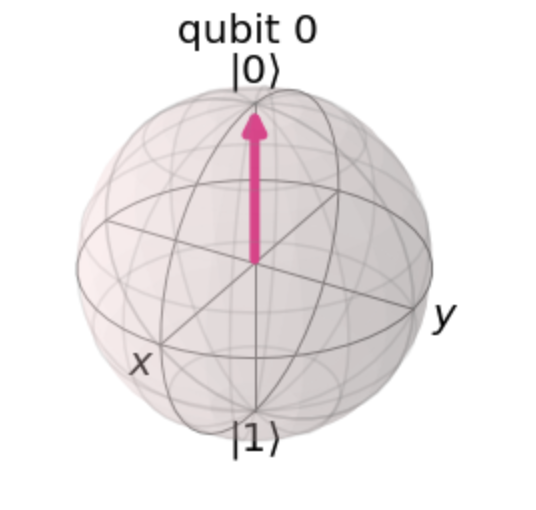
\includegraphics[width=\textwidth]{lab2/images/bSphX1.png}
        \caption{}
        \label{fig:bSphXY1}
    \end{subfigure}
    \hspace{0.2\textwidth}
    \begin{subfigure}[h]{0.33\textwidth}
        \centering
        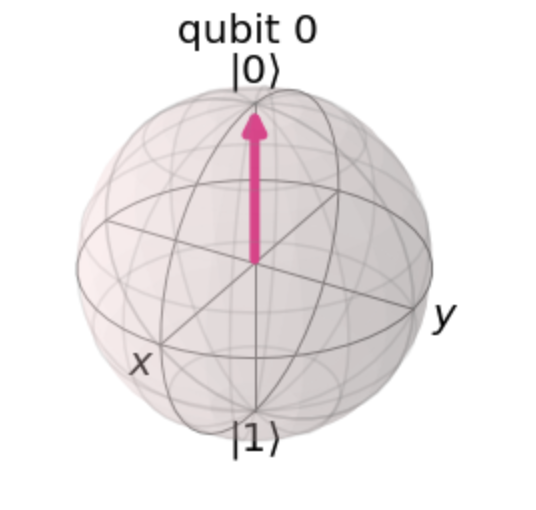
\includegraphics[width=\textwidth]{lab2/images/bSphX1.png}
        \caption{}
        \label{fig:bSphXY2}
    \end{subfigure}
    \caption{Bloch sphere showing a) the state of the initialised qubit and b) the state of the qubit after being passed through a Pauli-X gate and a Pauli-Y gate} 
    \label{fig:xyGateBloc}
\end{figure}

The reason for this is explained below:
\begin{enumerate}
    \item The qubit was initialised 
    \begin{enumerate}
        \item in state $|0\rangle$
    \end{enumerate}
    \item The X gate rotated this by $\pi$ around the x-axis of the Bloch sphere
    \begin{enumerate}
        \item resulting with a qubit in state $|1\rangle$
    \end{enumerate}
    \item The Y gate then rotated this by $\pi$ around the y-axis of the Bloch sphere
    \begin{enumerate}
        \item resulting in the qubit being in state $|0\rangle$
    \end{enumerate} 
\end{enumerate}

\subsection{The Hadamard Gate}\label{sec:HZH}
The Hadamard gate (H gate) is a fundamental quantum gate, represented by the following matrix:

$$ H = \tfrac{1}{\sqrt{2}}\begin{bmatrix} 1 & 1 \\ 1 & -1 \end{bmatrix} $$

It allows states to occupy a superposition of $|0\rangle$ and $|1\rangle$:

$$ H|0\rangle = \tfrac{1}{\sqrt{2}}\begin{bmatrix} 1 & 1 \\ 1 & -1 \end{bmatrix}\begin{bmatrix} 1 \\ 0 \end{bmatrix} = \tfrac{1}{\sqrt{2}} \begin{bmatrix} 1 \\ 1 \end{bmatrix}= |+\rangle 
\quad \quad \quad \quad 
H|1\rangle = \tfrac{1}{\sqrt{2}}\begin{bmatrix} 1 & 1 \\ 1 & -1 \end{bmatrix}\begin{bmatrix} 0 \\ 1 \end{bmatrix} = \tfrac{1}{\sqrt{2}} \begin{bmatrix} 1 \\ -1 \end{bmatrix}= |-\rangle $$

The H gate can transform the state of the qubit between the X and Z bases. It essentially performs a rotation around the Bloch vector `[1,0,1]' (the line between the x and z-axis).

Applying the sequence of gates: HZH, to any qubit state is equivalent to applying a single X-gate, shown mathematically below.

$$ H = \tfrac{1}{\sqrt{2}}\begin{bmatrix} 1 & 1 \\ 1 & -1 \end{bmatrix} \quad\quad  Z = \begin{bmatrix} 1 & 0 \\ 0 & -1 \end{bmatrix} \quad\quad  X = \begin{bmatrix} 0 & 1 \\ 1 & 0 \end{bmatrix} $$

\begin{equation*} 
\begin{split}
HZH & = \tfrac{1}{\sqrt{2}}\begin{bmatrix} 1 & 1 \\ 1 & -1 \end{bmatrix} \begin{bmatrix} 1 & 0 \\ 0 & -1 \end{bmatrix}\tfrac{1}{\sqrt{2}}\begin{bmatrix} 1 & 1 \\ 1 & -1 \end{bmatrix} \\
HZH & = \tfrac{1}{\sqrt{2}}\tfrac{1}{\sqrt{2}}\begin{bmatrix} 1 & 1 \\ 1 & -1 \end{bmatrix} \begin{bmatrix} 1 & 0 \\ 0 & -1 \end{bmatrix}\begin{bmatrix} 1 & 1 \\ 1 & -1 \end{bmatrix} \\
HZH & = \tfrac{1}{2}\begin{bmatrix} 1 & -1 \\ 1 & 1 \end{bmatrix}\begin{bmatrix} 1 & 1 \\ 1 & -1 \end{bmatrix}\\
HZH & = \tfrac{1}{2}\begin{bmatrix} 0 & 2 \\ 2 & 0 \end{bmatrix} \\
HZH & = \begin{bmatrix} 0 & 1 \\ 1 & 0 \end{bmatrix} \\
HZH & = X
\end{split}
\end{equation*}

The following circuit was written to verify this.

\begin{figure}[h]
    \centering
    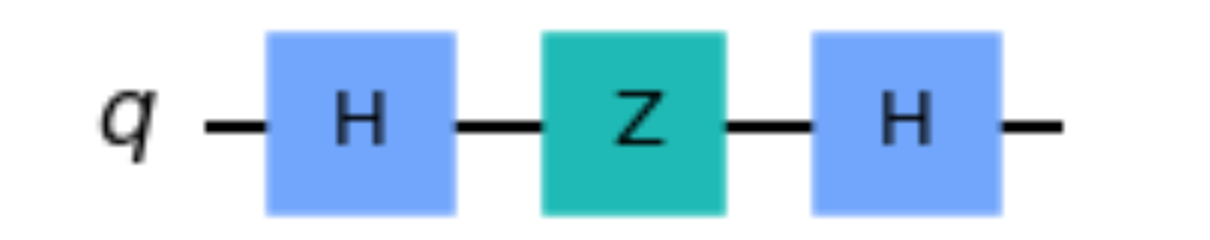
\includegraphics[width=0.4\textwidth]{lab2/images/hzhCircuit.png}
    \caption{Circuit diagram of a Hadamard gate, followed by a Pauli-Z gate, followed by another Hadamard gate in series} 
    \label{fig:hzhCircuit}
\end{figure}

The resultant state of the qubit after being passed through the circuit shown in Figure \ref{fig:hzhCircuit} was observed using a Bloch sphere:

\begin{figure}[h]
    \centering
    \begin{subfigure}[h]{0.24\textwidth}
        \centering
        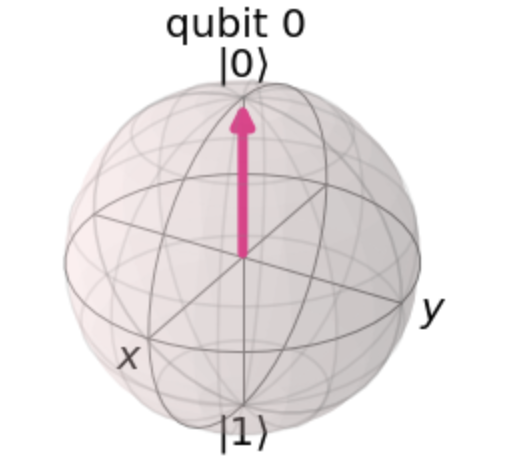
\includegraphics[width=\textwidth]{lab2/images/hzhGate1.png}
        \caption{Initial state}
        \label{fig:hzhGate1}
    \end{subfigure}
    \hfill
    \begin{subfigure}[h]{0.24\textwidth}
        \centering
        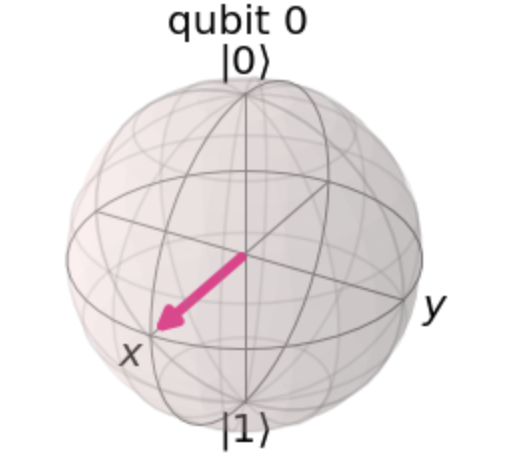
\includegraphics[width=\textwidth]{lab2/images/hzhGate2.png}
        \caption{After H gate}
        \label{fig:hzhGate2}
    \end{subfigure}
        \begin{subfigure}[h]{0.24\textwidth}
        \centering
        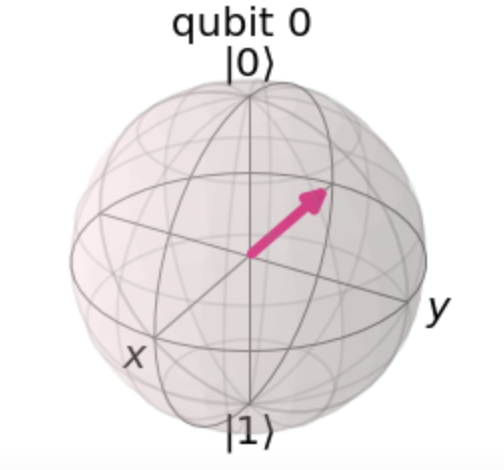
\includegraphics[width=\textwidth]{lab2/images/hzhGate3.png}
        \caption{After Z gate}
        \label{fig:hzhGate3}
    \end{subfigure}
        \begin{subfigure}[h]{0.24\textwidth}
        \centering
        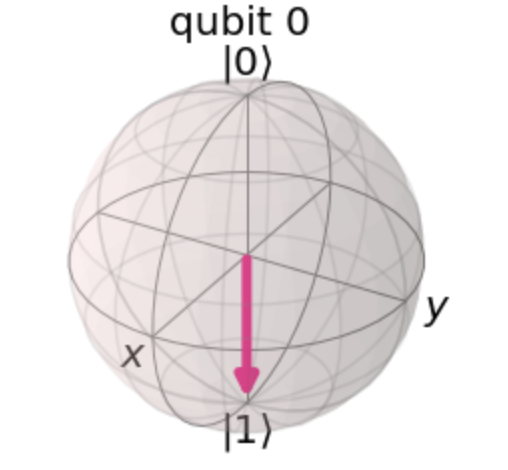
\includegraphics[width=\textwidth]{lab2/images/hzhGate4.png}
        \caption{After H gate}
        \label{fig:hzhGate4}
    \end{subfigure}
    \caption{Bloch sphere showing the state of the qubit after each gate is applied} 
    \label{fig:bSphereHZHGate}
\end{figure}

It is clear upon comparing the initial state (Figure \ref{fig:hzhGate1}) to the final state (Figure \ref{fig:hzhGate4}) that applying the sequence of gates: HZH has an identical effect to applying a single X gate (see Figure \ref{fig:xyGateBloc}).

\subsection{Multi-Qubit Gates}

\subsubsection{The CNOT Gate}
The CNOT gate is a conditional two-qubit gate that performs an X gate on the second qubit (target), if the state of the first qubit (control) is  $|1\rangle$. The truth table for a CNOT gate is shown in the table below.

\begin{table}[h]
\centering
\begin{tabular}{cccc}
\multicolumn{2}{c}{Input}                         & \multicolumn{2}{c}{Output}   \\ 
\multicolumn{1}{c|}{Control} & \multicolumn{1}{c||}{Target} & \multicolumn{1}{c|}{Control} & Target \\ \hline\hline
\multicolumn{1}{c|}{0}  & \multicolumn{1}{c||}{0}  & \multicolumn{1}{c|}{0}  & 0  \\ \hline
\multicolumn{1}{c|}{0}  & \multicolumn{1}{c||}{1}  & \multicolumn{1}{c|}{0}  & 1  \\ \hline
\multicolumn{1}{c|}{1}  & \multicolumn{1}{c||}{0}  & \multicolumn{1}{c|}{1}  & 1  \\ \hline
\multicolumn{1}{c|}{1}  & \multicolumn{1}{c||}{1}  & \multicolumn{1}{c|}{1}  & 0 
\end{tabular}
\label{tab:cNotTruth}
\caption{Truth table for CNOT gate}
\end{table}

A 2-qubit quantum circuit was created, where the 2 qubits are entangled and the output was measured. The circuit diagram is shown in Figure \ref{fig:entangleMeasure}

\begin{figure}[h]
    \centering
    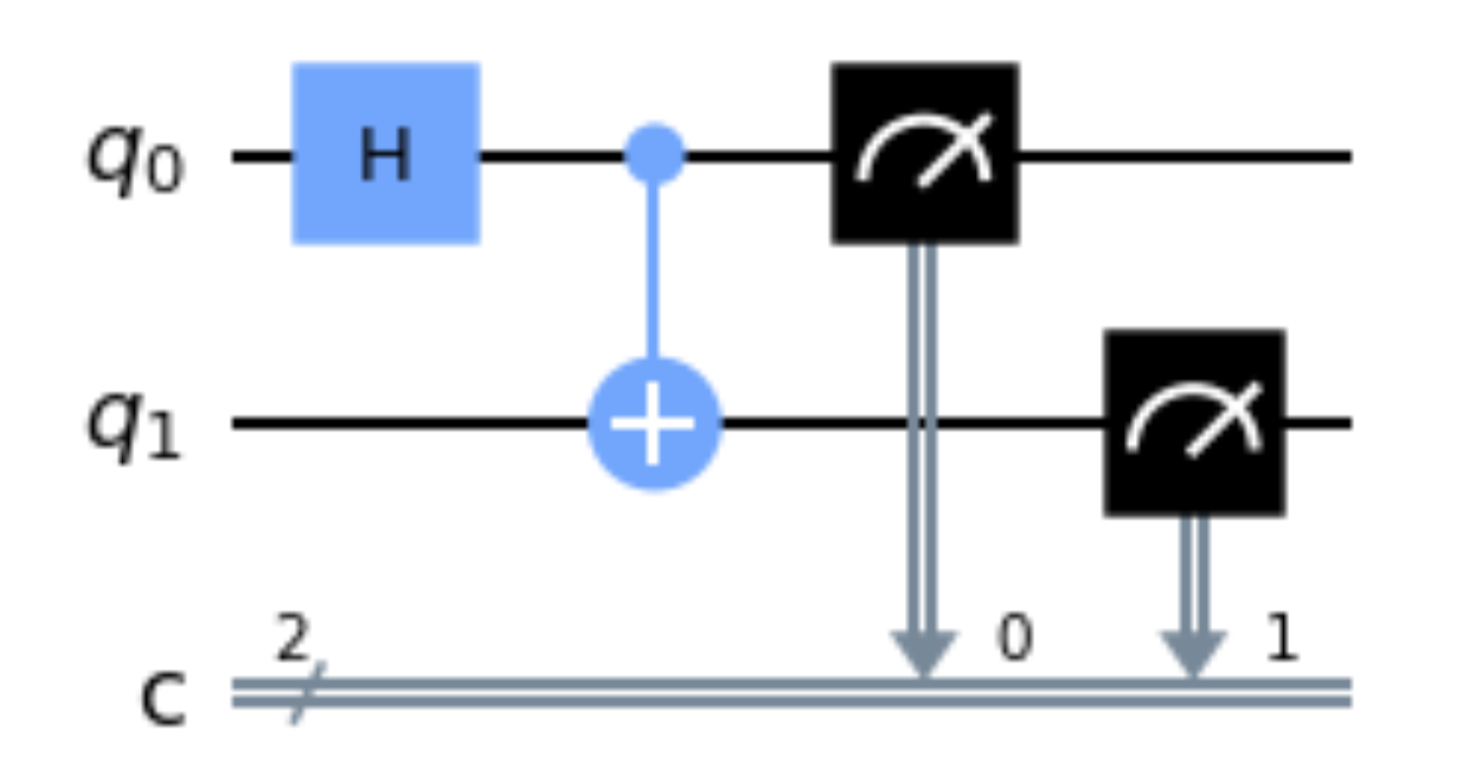
\includegraphics[width=0.4\textwidth]{lab2/images/entangleMeasure.png}
    \caption{Diagram of circuit for measuring entangled qubits} 
    \label{fig:entangleMeasure}
\end{figure}

Both qubits were initialised in state $|0\rangle$. The H gate transformed q$_0$ from state $|0\rangle$ into a superposition of state $|0\rangle$ and $|1\rangle$. This means, when measuring q$_0$, 50\% of the time the qubit will collapse into state $|0\rangle$, otherwise it will collapse into state $|1\rangle$. q$_0$ was then used as a control bit, meaning half of the time it switches the q$_1$ to state $|1\rangle$; the other half q$_1$ will remain unchanged in state $|0\rangle$. As a result, two possible outcomes are expected from this circuit:
\begin{itemize}
    \item 50\% of the time the output is expected to be in state $|00\rangle$
    \item 50\% of the time the output is expected to be in state $|11\rangle$
\end{itemize}

This was circuit was simulated, the results of which are shown in Figure \ref{fig:qiskitHistogram}. The simulation was run 1024 times: 49\% of the time the output was in state $|00\rangle$, and 51\% of the time the output was in state $|11\rangle$ -- not a 50/50 split as expected. This is discussed further in Section \ref{sec:comparison}. To determine a realistic response IBMs quantum computer was used. The results, again, were not in complete agreement with the theory, shown in Figure \ref{fig:ibmHistogram}. An explanation for this can be found in Section \ref{sec:discussion}.

\begin{figure}[h]
    \centering
    \begin{subfigure}[h]{0.5\textwidth}
        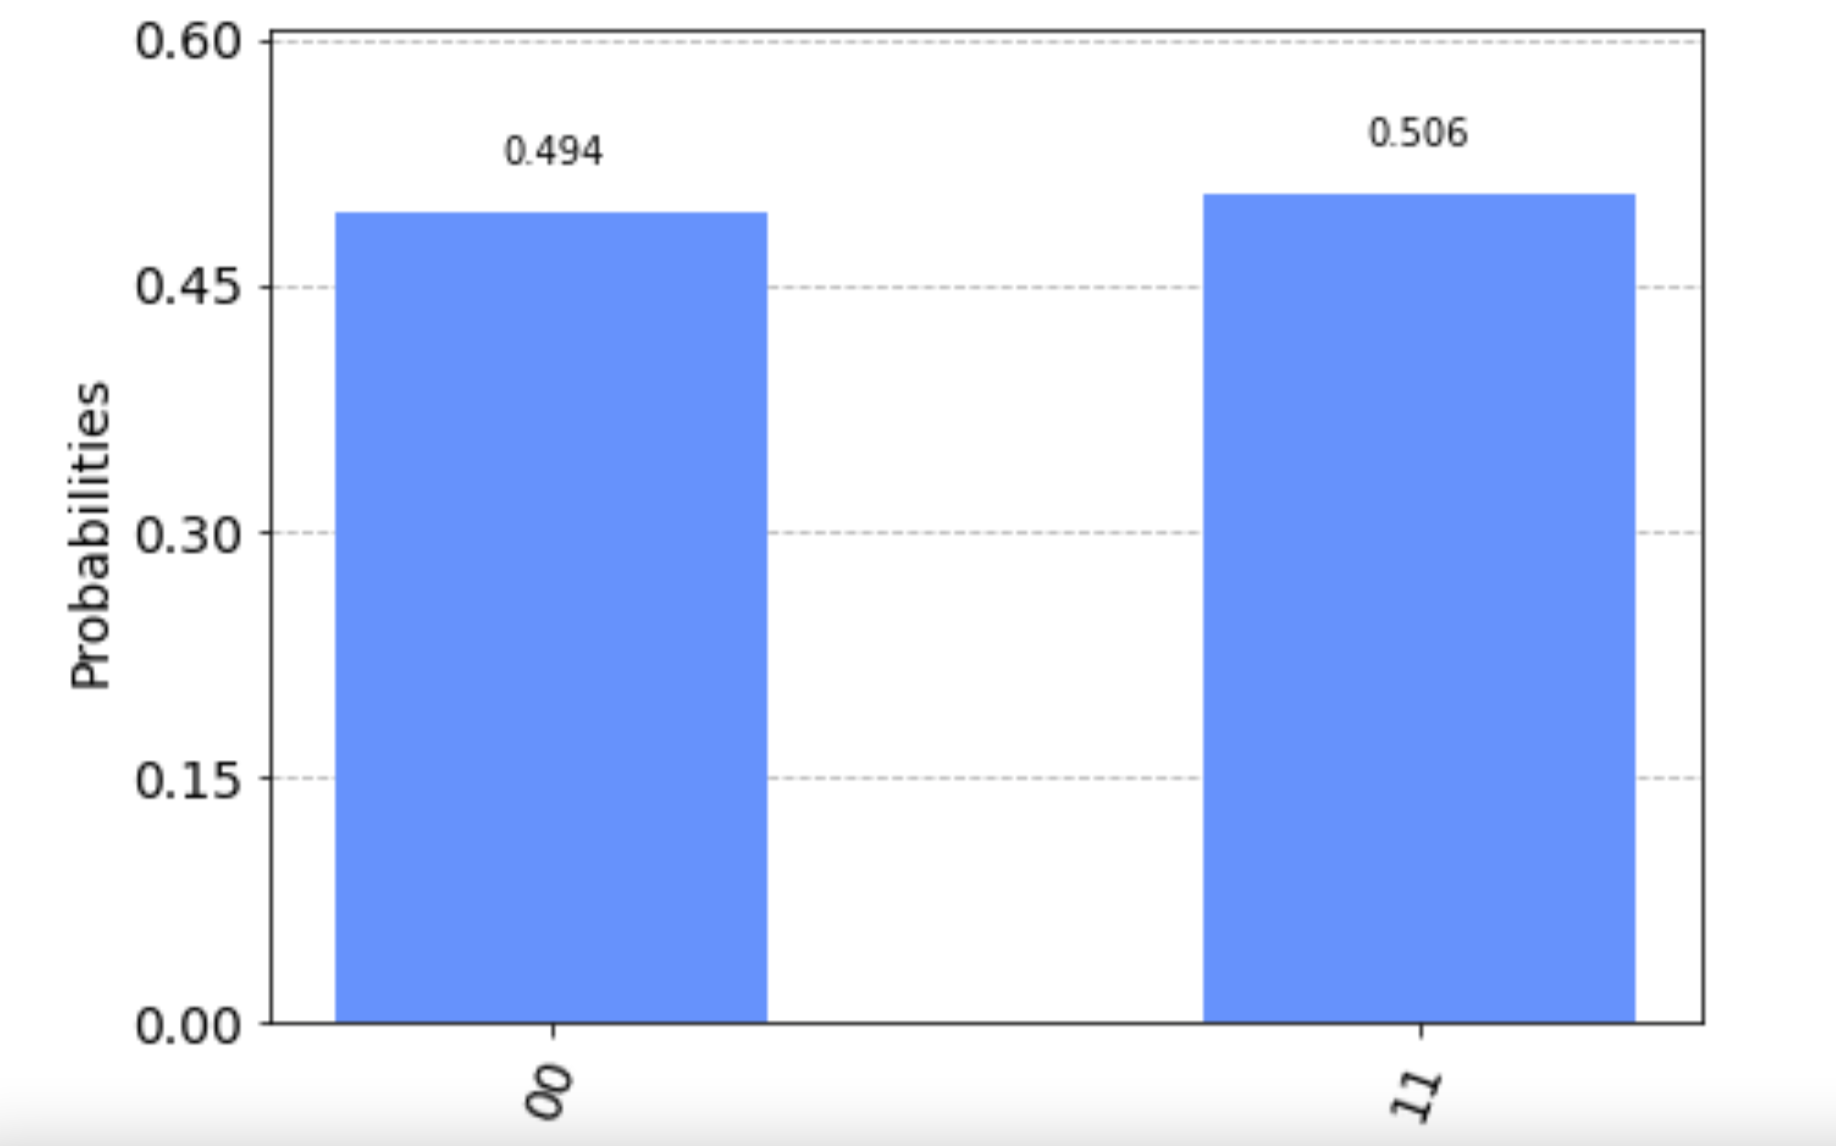
\includegraphics[width=\textwidth]{lab2/images/qiskitHistogram.png}
        \caption{} 
        \label{fig:qiskitHistogram}
    \end{subfigure}
    \hfill
    \begin{subfigure}[h]{0.43\textwidth}
        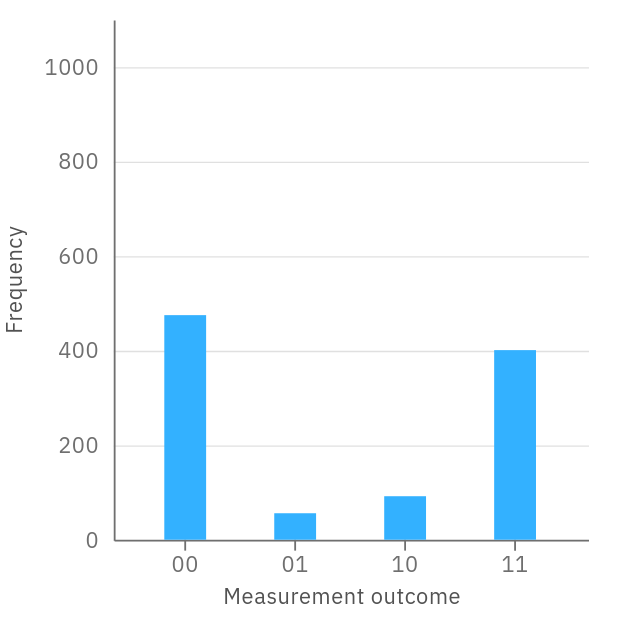
\includegraphics[width=\textwidth]{lab2/images/ibmHistogram.png}
        \caption{} 
        \label{fig:ibmHistogram}
    \end{subfigure}
    \caption{Histogram showing a) the probability of measuring each possible state according to qiskit and b) the frequency of the states measured after implementing the circuit using IBM's quantum computer} 
    \label{fig:hisogram}
\end{figure}

\section{Comparison of Results with Theory} \label{sec:comparison}
%Needs a breif read through
In general the results were consistent with the theoretical predictions, however, as soon as measurements were taken the outcome was slightly different as expected. For example, the histogram shown in Figure \ref{fig:qiskitHistogram} shows a 49/51 split in results (not 50/50 split as expected). This is because the Aer simulator was used which introduces noise. `Noise' describes all of the things that cause interference in a quantum computer, thus, the ideal case is no longer being considered. In reality, a quantum computer is susceptible to interference from all sorts of sources, like electromagnetic signals, 
disturbances in the Earth’s magnetic field. When qubits in a quantum computer are exposed to this kind of noise, the information in them gets degraded. This noise resulted in the degradation of the information in the qubits which added error into the system, meaning there was not an exact 50/50 split in the output. producing error in the system into not exactly 50/50. This can be improved by increasing the number of `shots' -- by increasing the number of times the simulation is run, the outcome is more likely to be closer to the probability stated by the mathematics -- however, some percentage of noise is unavoidable.

\section{Discussion} \label{sec:discussion}
\textbf{Question 1:}

Initialise a qubit, and apply the X gate to it. Confirm your result by drawing the circuit and visualising the flipped state using the Block sphere (use/copy and paste the examples above wherever appropriate).

Circuit diagram of X gate shown in Figure \ref{fig:xGate} with Bloch sphere visualising states shown in Figure~\ref{fig:bSphereXGate}.

\textbf{Question 2:}
Apply the x and y gates to the qubit above and draw it on your screen.

Circuit diagram of X and Y gate shown in Figure \ref{fig:xyGateDiagram} with Bloch sphere visualising states shown in Figure~\ref{fig:xyGateBloc}.

\textbf{Question 3:}
Show mathematically that applying the sequence of gates: HZH, to any qubit state is equivalent to applying an X gate. Then, write a circuit that will show this (you can check each step/rotation, by plotting the new state on the Bloch Sphere each time.

Mathematical proof can be found in Section \ref{sec:HZH}. The circuit diagram and Bloch sphere visualising the states is shown in Figure \ref{fig:hzhCircuit} and \ref{fig:bSphereHZHGate} respectively.

\textbf{Question 4:}
Build a 2-qubit quantum circuit where the 2 qubits are entangled and measure the output. Does this agree with the mathematical prediction? If not, why would you say that is so

Circuit diagram for measuring entangled qubits is shown in Figure \ref{fig:entangleMeasure}. The results did not agree with the mathematical prediction, a 50/50 split in output was expected. The reasoning for this is discussed in Section \ref{sec:comparison}.

\textbf{Question 5:}
Use IBM composer and compare its results to what you obtained above. Are they different? How so? Is there anything you can do to make the results come closer to the mathematical expectation?

The circuit shown in Figure \ref{fig:entangleMeasure} was implemented in IBMs quantum computer, results of which can be found in Figure \ref{fig:ibmHistogram}. It is clear that the final state was not 50/50 split between state $|00\rangle$ and $|11\rangle$, as predicted by the mathematics. In fact, occasionally the final state was found to be in state $|01\rangle$ and $|10\rangle$. This is because qubits are very fragile and are prone to errors and other quantum noise. The characteristics that make quantum systems powerful also makes them delicate. Disturbances among qubits can corrupt the state of the qubits and cause errors such as bit flip errors -- an error where the qubits computational state flips from 1 to 0 or vice versa. This explains why occasionally the system was measured to be in state $|01\rangle$ and $|10\rangle$. These errors can be reduced by employing error correction algorithms. In addition to building qubits that are physically less prone to mistakes, scientists often hope to implement quantum error correction (QEC) -- compensate for high error rates by spreading quantum information across many redundant qubits. QEC is used in quantum computing to protect quantum information from errors due to decoherence and other quantum noise. Quantum error correction is essential if one is to achieve fault-tolerant quantum computation that can deal not only with noise on stored quantum information. Another reason for the error could be due to faulty measurements. Measurements generally disturb quantum systems. The disturbance caused by measurement depends on the details of the interaction between system and apparatus; this can generally be improved by increasing the number of shots.

\section{Conclusions}

In this lab, quantum circuits were implemented and visualised using qiskit. Through the use of circuit diagrams and Bloch sphere's, a deeper understanding of quantum gates and quantum operations was achieved. The objectives were fulfilled with ease, therefore I do not believe any changes are necessary to attain them.

The Pauli gates were inspected and represented in a familiar setting -- the circuit diagrams were similar to the classical circuit diagrams. The Hadamard gate was also considered, which can be used to transform a qubit from a $|0\rangle$ or $|1\rangle$ state to a state of superposition (or vice versa) -- the Bloch sphere helped visualise this. Finally, the CNOT gate was considered, and was used to entangle two qubits together. By comparing the results from qiskit to an actual quantum computer a greater understanding of quantum systems was achieved. I believe this lab was an excellent introduction to quantum circuits as I understood how quantum gates work and how they can be used to create quantum circuits.